% Week 5 report for the QSVM track, structured as a scientific paper.
%
% Build:  latexmk -pdf qsvm_week5_report.tex
%
% Figures are vector PDFs under figures/, generated by
%   uv run python scripts/make_report_figures.py
% Regenerate them rather than editing them.
%
% Scope: this report presents results and the limitations OF THOSE RESULTS.
% Work that was never carried out is tracked in NOTES_open_items.md and is
% deliberately absent here.

\documentclass[11pt]{article}

\usepackage[a4paper,margin=1in]{geometry}
\usepackage{lmodern}
\usepackage[T1]{fontenc}
\usepackage[utf8]{inputenc}
\usepackage{amsmath,amssymb}
\usepackage{booktabs}
\usepackage{graphicx}
\usepackage{caption}
\usepackage{siunitx}
\usepackage[hidelinks]{hyperref}
\usepackage{microtype}
\usepackage{enumitem}

\captionsetup{font=small,labelfont=bf}
\sisetup{detect-weight=true,detect-inline-weight=math}
\setlist{itemsep=1pt,topsep=3pt}

\newcommand{\nc}{\ensuremath{n_{\mathrm{components}}}}
\newcommand{\best}[1]{\textbf{#1}}

\title{Isolating the cause of quantum-kernel failure on\\
malware family attribution\\[0.3em]
\large Complete classical baselines, subsample validation,\\
kernel diagnostics and paired significance tests}
\date{2 August 2026}

\begin{document}
\maketitle

\begin{abstract}
\noindent
\textbf{Background.} A fidelity-kernel quantum support vector machine (QSVM) had
been observed to fall to the chance level on the 15-class task of CIC-MalMem-2022
while performing well above chance on the equivalent EMBER 2018 task. Class
imbalance and qubit count had been excluded, and the cause was unidentified. The
classical arm of the comparison on EMBER used a single model, and no difference
between the two frameworks had been tested statistically.

\noindent
\textbf{Methods.} We complete the EMBER classical baseline with four models at
$\nc{} \in \{1,3,6\}$ on both tasks, validate the 1000-row subsample on which all
quantum results rest, measure class separability of the shared PCA projection,
and measure kernel concentration and kernel-target alignment against a classical
RBF control built on the identical feature matrix. Every quantum--classical pair
with a complete cross-validation sweep is tested with a paired $t$-test.

\noindent
\textbf{Results.} Random forest beats SVM on every EMBER binary configuration, so
the previously reported classical advantage was understated by $0.011$ to
$0.027$ macro-F1. Both subsamples are faithful, with Kolmogorov--Smirnov
rejection counts far below their null expectations. EMBER's families are
$\approx 8\times$ more separable than CIC's, which accounts for poor absolute
performance but not for a QSVM-specific deficit. The RBF control produces the
same off-diagonal Gram spread on both corpora ($0.2212$ against $0.2184$),
whereas the fidelity kernel matches RBF on EMBER ($0.92\times$) and collapses to
$0.40\times$ on CIC. All 84 comparable pairs favour the classical model at
$p<0.05$.

\noindent
\textbf{Conclusions.} The QSVM's collapse on CIC is attributable to kernel
concentration rather than to feature difficulty, and it is a property of the
kernel rather than of the corpus.
\end{abstract}

\section{Introduction}

A fidelity-kernel QSVM had been compared against classical baselines on two
malware corpora under a protocol that equalises rows, cross-validation folds and
input dimensionality between the two arms. Three questions were left open by that
comparison.

First, the EMBER classical arm used a support vector machine only, so every
recorded margin there was a comparison against one baseline rather than against
the strongest available. Second, the QSVM fell to the chance level on CIC
15-class while reaching $0.42$--$0.52$ macro-F1 on EMBER 15-class, and the cause
was unidentified after class imbalance and qubit count had been excluded. Third,
every claim of a classical advantage rested on differences in mean macro-F1 with
no test that any gap exceeded fold-to-fold noise. A fourth, quieter issue was
that all quantum results are computed on a 1000-row subsample whose fidelity to
its population had been assumed rather than measured.

This report addresses all four. Its central contribution is a diagnosis: by
building a classical RBF kernel on the identical feature matrix, we separate the
hypothesis that CIC's features are hard from the hypothesis that the fidelity
kernel fails on them, and find for the latter.

\subsection*{Progress this week}

\begin{center}
\small
\begin{tabular}{@{}llp{0.50\textwidth}@{}}
\toprule
\textbf{Day} & \textbf{Work} & \textbf{Outcome} \\
\midrule
29 & EMBER four-model classical baseline
   & Classical advantage on binary widened by $0.011$ to $0.027$ macro-F1 \\
30 & Third-corpus scope decision
   & Recorded separately from this report \\
31 & Subsample validation and class separability
   & Subsamples verified faithful; separability gap quantified \\
32 & ---
   & Outside this track \\
33 & Kernel concentration and target alignment
   & Collapse mechanism identified against an RBF control \\
34 & Paired significance tests and master tables
   & 84 of 84 comparable pairs at $p<0.05$ \\
35 & Consolidation
   & Reports and paper sections written \\
\bottomrule
\end{tabular}
\end{center}

Six of the seven scheduled days fall inside this track and all six are complete.
The week added 90 cross-validation fold runs to the experiment log, bringing it
to 976, and the implementation carries 149 passing tests. Three of the six days
changed a previously published conclusion rather than extending it: the
completed baseline on day 29, the mechanism on day 33, and the significance
tests on day 34.

\section{Materials and methods}
\label{sec:methods}

\subsection{Data}

Two corpora, each with a binary detection task and a 15-class family attribution
task.

\begin{description}[leftmargin=1.2em,style=nextline]
\item[CIC-MalMem-2022] Obfuscated-malware memory dumps, 55 numeric forensic
features. Binary: all \num{58596} rows, balanced. 15-class: \num{29298}
malware-only rows over 15 families, $1.7\times$ imbalanced.
\item[EMBER 2018] Static portable-executable features, 2381 dimensions, on an
\num{18014}-row extract of the published test set. Binary: all \num{18014} rows,
$88.9\%$ malware. 15-class: \num{14325} rows balanced at 955 per family.
\end{description}

\subsection{Shared protocol}

Both frameworks consume one feature pipeline: a zero-variance filter, a
correlation filter at $0.95$, standardisation, then PCA to \nc{} components, fit
on training-fold rows only. \nc{} is the single alignment point, setting the
classical feature count and the quantum qubit budget simultaneously.

The fidelity kernel costs one circuit evaluation per pair of training samples, so
quantum runs use a stratified 1000-row subsample. That subsample and its five
stratified outer folds are written to disk by the quantum runner and reloaded by
the classical runner, so both are scored on identical rows and folds, with 800
training and 200 held-out rows per fold.

All results are held-out macro-F1 averaged over the five outer folds.
Hyperparameters are tuned by an Optuna inner loop inside each training fold.
Accuracy is not reported: on EMBER binary at $\nc{}=1$ the QSVM attains $0.890$
accuracy in three of five folds while the benign class's F1 is exactly $0.000$,
because $88.9\%$ of rows are malware and the model labels everything malware.

\subsection{Measurements introduced here}

\begin{description}[leftmargin=1.2em,style=nextline]
\item[Complete classical baseline] Random forest, XGBoost and LightGBM added
alongside the existing SVM at $\nc{} \in \{1,3,6\}$ on both EMBER tasks, replaying
the persisted quantum splits.
\item[Subsample representativeness] Per-class proportion drift, per-feature mean
and standard-deviation drift, and a per-feature two-sample Kolmogorov--Smirnov
test of the 1000-row subsample against its full population, with the rejection
count read against its null expectation $\alpha \cdot n_{\mathrm{features}}$.
\item[Class separability] One-vs-rest Fisher discriminant ratio, silhouette
coefficient, pairwise centroid distance and cumulative explained variance of the
shared PCA projection, fit on training-fold rows only.
\item[Kernel diagnostics] Off-diagonal standard deviation of the training Gram
(concentration) and Frobenius kernel-target alignment
$\langle K, YY^{\!\top}\rangle_F / (\lVert K\rVert_F \lVert YY^{\!\top}\rVert_F)$,
measured for the fidelity kernel and for an RBF kernel built on the identical
post-PCA feature matrix.
\item[Paired significance] A paired $t$-test and a Wilcoxon signed-rank test over
the five per-fold macro-F1 values for every quantum--classical pair with a
complete sweep.
\end{description}

\subsection{Selection of comparable runs}
\label{sec:selection}

Runs are grouped by cross-validation sweep rather than by configuration. The same
configuration was swept more than once, so a parameter-based grouping returns 10,
15 or 20 records for a five-fold sweep and averages distinct hyperparameter
searches together; 57 parameter groups in the experiment log have a size other
than five. For the QSVM the encoding is additionally a \emph{per-fold outcome}
rather than a configuration key, because the tuner selects it inside each fold,
so one sweep tuning over both encodings can appear as four angle folds and one
IQP fold. Fold records are therefore grouped by parent run, retaining only sweeps
that completed with exactly five folds. Under that rule the log holds 125 nested
sweeps, 123 of them complete.

\section{Results}
\label{sec:results}

\subsection{The classical baseline was incomplete}

\begin{table}[htbp]
\centering
\small
\caption{EMBER 2018, held-out macro-F1, mean over five outer folds. Best
classical model in bold.}
\label{tab:ember}
\begin{tabular}{@{}l S[table-format=1.4] S[table-format=1.4] S[table-format=1.4]
S[table-format=1.4] S[table-format=1.4] S[table-format=1.4]@{}}
\toprule
& {Random forest} & {XGBoost} & {LightGBM} & {SVM} & {QSVM angle} & {QSVM IQP} \\
\midrule
\multicolumn{7}{@{}l}{\emph{Binary}}\\
$\nc{}=1$ & \best{0.5582} & 0.5451 & 0.5093 & 0.5314 & 0.4532 & 0.4587 \\
$\nc{}=3$ & \best{0.6575} & 0.6465 & 0.6434 & 0.6306 & 0.4924 & 0.5084 \\
$\nc{}=6$ & \best{0.6835} & 0.6680 & 0.6593 & 0.6724 & 0.5138 & 0.5137 \\
\addlinespace
\multicolumn{7}{@{}l}{\emph{15-class}}\\
$\nc{}=1$ & \best{0.5562} & 0.5313 & 0.5410 & 0.5294 & 0.1688 & 0.1541 \\
$\nc{}=3$ & 0.7194 & 0.7089 & 0.7035 & \best{0.7389} & 0.3908 & 0.4797 \\
$\nc{}=6$ & 0.7903 & 0.7659 & 0.7709 & \best{0.7930} & 0.4232 & 0.5195 \\
\bottomrule
\end{tabular}
\end{table}

Random forest beats SVM on every binary configuration (Table~\ref{tab:ember}), so
the classical advantage widens from $+0.0727$ to $+0.0995$ at $\nc{}=1$, from
$+0.1222$ to $+0.1491$ at $\nc{}=3$, and from $+0.1587$ to $+0.1697$ at
$\nc{}=6$. On the 15-class task SVM is the strongest baseline at
$\nc{} \in \{3,6\}$, so those margins are unchanged. Four of six configurations
move, and all four move in the same direction.

\begin{figure}[htbp]
\centering
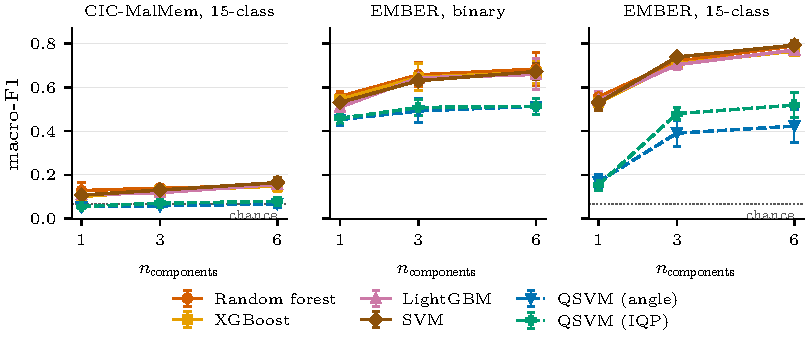
\includegraphics[width=\textwidth]{figures/fig_capacity_scaling.pdf}
\caption{Macro-F1 against the shared feature and qubit budget. Solid lines are
classical, dashed lines the two QSVM encodings. Error bars are one standard
deviation over the five outer folds, and the dotted line marks the 15-class
chance level. CIC binary is not shown because its sweeps are not separable
(§\ref{sec:limits}).}
\label{fig:capacity}
\end{figure}

Figure~\ref{fig:capacity} shows the trend with capacity. On EMBER binary the QSVM
gains $0.055$ macro-F1 from one to six components where the random forest gains
$0.125$, so the gap widens rather than closing.

\subsection{The subsample preserves its population}

\begin{figure}[htbp]
\centering
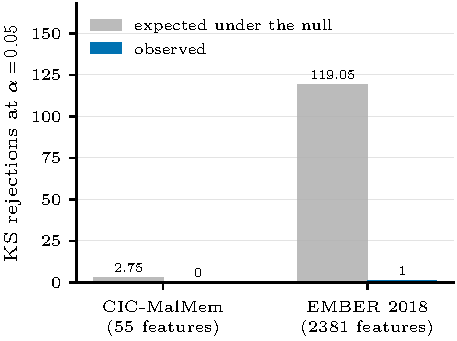
\includegraphics[width=0.55\textwidth]{figures/fig_representativeness.pdf}
\caption{Per-feature Kolmogorov--Smirnov rejections at $\alpha=0.05$, 1000-row
subsample against full population, beside the count chance alone produces.}
\label{fig:repr}
\end{figure}

A rejection count is interpretable only against its null expectation, since a
faithful subsample still rejects about $\alpha \cdot n_{\mathrm{features}}$
features by chance. CIC rejects 0 of 55 features where $\approx 2.75$ were
expected, and EMBER 1 of 2381 where $\approx 119$ were expected
(Figure~\ref{fig:repr}). Maximum class-proportion drift is below $0.001$ on both,
and maximum per-feature mean drift is $0.046$ and $0.122$ population standard
deviations respectively.

\subsection{Feature geometry accounts for the corpus, not the kernel}

\begin{figure}[htbp]
\centering
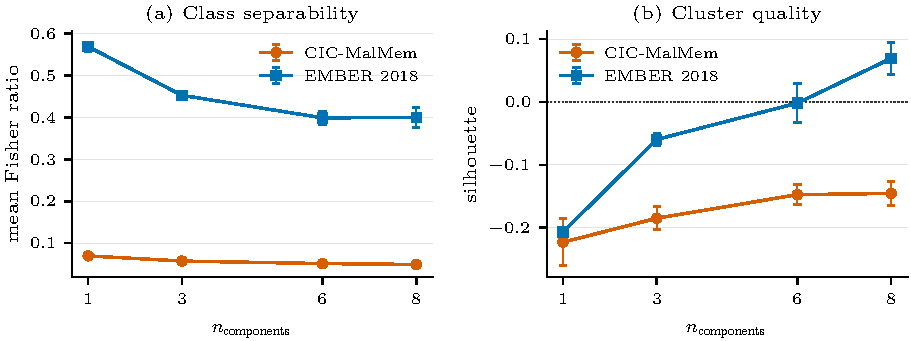
\includegraphics[width=\textwidth]{figures/fig_geometry.pdf}
\caption{Class separability of the shared PCA projection, averaged over the five
outer folds. Both metrics are scale-invariant and therefore comparable across
corpora of very different dimensionality.}
\label{fig:geom}
\end{figure}

EMBER's families are $\approx 8\times$ more separable by one-vs-rest Fisher ratio
and up to $50\times$ on the worst-case family (Figure~\ref{fig:geom}). CIC's
silhouette coefficient is negative at every \nc{}, so the average point lies
closer to another family's centroid than to its own. CIC's PCA nonetheless
explains substantially more variance ($33$--$81\%$ against $8$--$30\%$), placing
its variance in directions that do not discriminate family.

This accounts for the poor absolute performance of every method on CIC 15-class.
It does not account for a QSVM-specific deficit, since a classical SVM extracts
$0.108$--$0.165$ macro-F1 from these same features where the QSVM extracts
$0.056$--$0.079$.

\subsection{Kernel concentration accounts for the kernel}
\label{sec:kernel}

\begin{figure}[htbp]
\centering
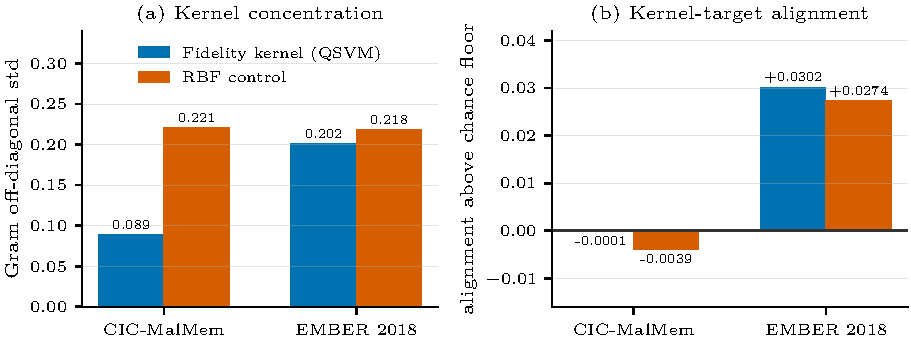
\includegraphics[width=\textwidth]{figures/fig_kernel_diagnostics.pdf}
\caption{First outer training fold, $\nc{}=6$, IQP encoding, 800 rows, with an RBF
control built on the identical feature matrix. (a) Off-diagonal Gram spread.
(b) Kernel-target alignment relative to its floor: a constant kernel scores
$1/\sqrt{15}\approx 0.258$ on 15 balanced classes, so only the excess is
informative.}
\label{fig:kernel}
\end{figure}

The RBF control produces near-identical off-diagonal spread on both corpora,
$0.2212$ against $0.2184$, so CIC's features do not cause a classical kernel to
concentrate. The fidelity kernel tracks RBF on EMBER at $0.92\times$ and collapses
to $0.40\times$ on CIC, compressing every off-diagonal similarity into a band
$2.5\times$ narrower from the same inputs and driving the Gram toward a scaled
identity.

Alignment behaves differently. On CIC the fidelity kernel lands $0.000069$
\emph{below} the constant-kernel floor, making it indistinguishable from a matrix
of ones, and the RBF control is also below it; on EMBER both clear the floor by
$\approx 0.03$. Alignment therefore separates the two corpora while concentration
separates the two kernels.

\begin{table}[htbp]
\centering
\small
\caption{Off-diagonal Gram spread across the 15-class sweep, mean over five outer
folds. These values were recorded on every fit, so no additional computation was
required.}
\label{tab:conc}
\begin{tabular}{@{}l S[table-format=1.4] S[table-format=1.4]
S[table-format=1.4] S[table-format=1.4]@{}}
\toprule
& {$\nc{}=1$} & {$\nc{}=3$} & {$\nc{}=6$} & {$\nc{}=8$} \\
\midrule
CIC, angle   & 0.1192 & 0.0795 & 0.0674 & 0.0600 \\
CIC, IQP     & 0.0927 & 0.1005 & 0.0882 & 0.0798 \\
EMBER, angle & 0.2044 & 0.1942 & 0.1363 & {---} \\
EMBER, IQP   & 0.1756 & 0.2569 & 0.2104 & {---} \\
\bottomrule
\end{tabular}
\end{table}

Table~\ref{tab:conc} confirms the effect is not an artefact of one fold or one
setting: EMBER's Gram is $1.9$--$2.6\times$ more spread than CIC's at every
comparable cell, and concentration worsens with qubit count on both, which is the
trend the bandwidth parameter exists to counteract.

\subsection{The differences are statistically significant}

\begin{figure}[htbp]
\centering
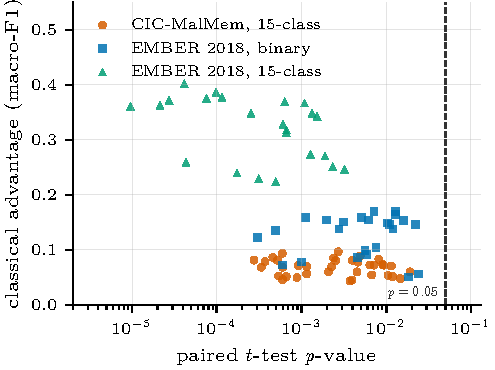
\includegraphics[width=0.56\textwidth]{figures/fig_significance.pdf}
\caption{Effect size against paired $t$-test $p$-value for all 84 comparable
quantum--classical pairs. Every point lies left of $p=0.05$ and above zero.}
\label{fig:sig}
\end{figure}

All 84 comparable pairs favour the classical model and all 84 reach $p<0.05$. The
largest $p$-value across every pair is $0.0241$ and the smallest is
$4 \times 10^{-6}$.

A Wilcoxon signed-rank test returns exactly $0.0625$ for all 84 pairs. With five
paired samples that is the smallest attainable two-sided $p$-value, so the test
cannot reach $0.05$ at this fold count regardless of effect size; all 84 reaching
the floor indicates that every pair achieved the most extreme rank configuration
available.

Among classical models on shared held-out predictions, McNemar's test separates
random forest from XGBoost on EMBER 15-class at $p=0.0022$, while on CIC 15-class
no pair of classical models separates at all, consistent with the geometry result
above.

\section{Discussion}

\subsection{Interpretation}

Three of the four open questions resolve cleanly. The classical baseline was
incomplete in a direction that understated the classical advantage; the subsample
underpinning every quantum result is faithful to its population; and the observed
differences are significant on every comparable pair rather than resting on mean
differences alone.

The fourth is the substantive finding. Feature geometry and kernel geometry give
different answers, and the difference is the diagnosis. Geometry explains why
every method performs poorly on CIC 15-class, since the projection places class
centroids closer to foreign points than to their own. It cannot explain a deficit
specific to the QSVM, because the classical SVM recovers two to three times the
QSVM's macro-F1 from the same projection. Kernel concentration does explain it:
the fidelity kernel loses $60\%$ of the RBF control's off-diagonal spread on
inputs where the control loses none. A Gram approaching a scaled identity
presents the support vector machine with a geometry in which all pairs are
equally similar, which is what a macro-F1 pinned to chance looks like internally.

The result is a statement about the method rather than the corpus, and it
predicts that the approach will degrade wherever the encoded states become
mutually near-orthogonal.

\subsection{Limitations}
\label{sec:limits}

\begin{description}[leftmargin=1.2em,style=nextline]
\item[Bandwidth is untested on CIC] Concentration is the identified mechanism and
bandwidth is the parameter that acts on it, but no bandwidth sweep was run.
§\ref{sec:kernel} identifies a mechanism; it does not demonstrate a remedy.
\item[Alignment is a weak predictor] Alignment reports that neither kernel carries
label information on CIC, yet a classical SVM reaches $0.16$ there. Alignment is a
global, unweighted average over all pairs, and a support vector machine requires
no such global property. It ranks corpus difficulty usefully and predicts
attainable SVM performance poorly. The concentration measurement does not share
this weakness, since it describes the matrix the SVM actually receives.
\item[Scope of the kernel measurement] The alignment and RBF-control figures come
from one training fold, one capacity and one encoding. Table~\ref{tab:conc} is
broader, spanning five folds, four capacities and both encodings, but carries no
RBF control. The RBF control itself uses a single unturned $\gamma$ heuristic, so
the comparison is against a reasonable classical default rather than the best
attainable classical kernel.
\item[One configuration is not separable] Every CIC binary run, classical and
quantum alike, predates sweep-level tracking in the experiment log and carries no
recoverable sweep boundary; 45 fold records per model resolve into two distinct
sweeps per \nc{} with no identifier separating them. No grouping was
reconstructed, since the time gaps between runs are not a recorded boundary. The
limitation is symmetric across frameworks, and it is why CIC binary is absent
from Figure~\ref{fig:capacity} and from the 84 tested pairs.
\item[No sample-level test between frameworks] McNemar's test requires per-sample
predictions from both models on a shared test set. QSVM predictions were not
persisted during the reported sweeps, so cross-framework evidence rests on five
paired fold-level scores.
\item[Fold count] Five outer folds support the paired $t$-test and are too few for
Wilcoxon, whose minimum attainable $p$-value at $n=5$ is $0.0625$. Six folds would
place $0.03125$ within reach.
\item[Simulator only] All quantum results use a state-vector simulator, with no
hardware execution and no noise model.
\end{description}

\subsection{Future work}

Sweep bandwidth on CIC, since the mechanism is identified and the corresponding
parameter has never been tuned there beyond its default. Move to six outer folds
so that a non-parametric test becomes usable.

\section{Conclusion}

Completing the classical baseline widened the recorded classical advantage on
EMBER binary by $0.011$ to $0.027$ macro-F1, and paired testing establishes that
all 84 comparable quantum--classical differences reach $p<0.05$. The 1000-row
subsample on which every quantum result depends is faithful to its population.

The QSVM's collapse to chance on CIC 15-class is attributable to kernel
concentration rather than to feature difficulty. A classical RBF kernel built on
the identical feature matrix retains its off-diagonal spread while the fidelity
kernel falls to $0.40\times$ of it, which locates the failure in the kernel and
names the parameter that acts on it.

\end{document}
